\section{Extraction de données}
\subsection{Web scraping}
\subsubsection{Qu'est ce que c'est ?}
Le web scraping est un processus automatisé de récupération de données à partir de site web sur Internet. Au moyen d'outils spécialisés, il permet une exploration systématique et une extraction ciblée d'informations à partir de la structure du site. Ces informations peuvent être textuelles, des images, vidéos ou autres.
\subsubsection{Outils}
Les outils de web scraping peuvent se ranger dans deux catégories :
\begin{itemize}
\item Les outils de scraping permettent de naviguer sur Internet pour aller chercher des données brutes (HTML, XML, PNG...). Quelques-uns des outils les plus employés en Python sont Requests, Selenium, Scrapy.
\item Les outils de parsing permettent de d'extraire de la donnée utilisable à partir des données brutes récupérées par le scraper. Beautiful Soup est une solution très populaire pour traiter les fichier au format HTML ou XML. Un autre module utilisé pour traiter les fichiers XML est ElementTree disponible en standard avec Python. Il est toutefois à utiliser avec prudence car il présente des vulnérabilités\cite{XMLProcessingModules}.
\end{itemize}

Les outils que nous avons retenus pour ce projet sont les bibliothèques Requests et Beautiful Soup.

\subsubsection{Comment procéder ?}

\paragraph{Scraping :}

Une première approche (illustrée figure \ref{naive}) montre que si le requêtage est facile à mettre en oeuvre, il est tout aussi facile à identifier comme illicite et à bloquer. Ici, le serveur a renvoyé le code 403 pour nous informer qu'il a bien compris notre requête mais a choisi de la bloquer.

\begin{center}
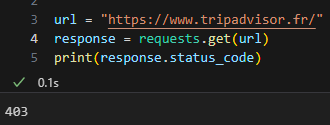
\includegraphics[scale=0.8]{Images/naive.png}
\captionof{figure}{Premier scraping, premier échec...}
\label{naive}
\end{center}

Cela vient du fait que lorsque nous avons soumis notre requête au serveur, nous avons omis de communiquer certaines information comme le veut le protocole HTTP.
\paragraph*{Le header} est un ensemble d'informations qui explicite le contexte de la communication attendue avec le serveur (Une liste des champs disponibles peut être consultée en ligne\cite{HTTPHeadersHTTP2024}). Un header est ainsi envoyé à un serveur à chaque fois que nous visitons un site web sur Internet. Il suffit d'utiliser les outils développeurs disponibles dans le navigateur pour le visualiser. 

\begin{center}
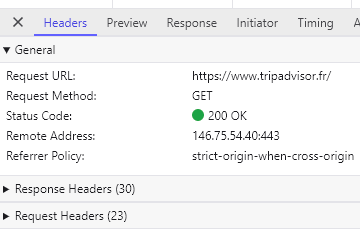
\includegraphics[scale=0.8]{Images/header.png}
\captionof{figure}{Header dans les outils développeurs (Brave)}
\label{header_Brave}
\end{center}

La figure \ref{header_Brave} montre que la requête du navigateur :
\begin{itemize}
\item portait sur la page https://www.tripadvisor.fr/
\item a utilisé la méthode GET
\item a été acceptée par le serveur (code 200 pour une requête acceptée, code 403 si elle est refusée)
\item contenait un header composé de 23 champs
\end{itemize}

Il est alors possible de copier ces informations et de les envoyer dans notre requête get.

\begin{center}
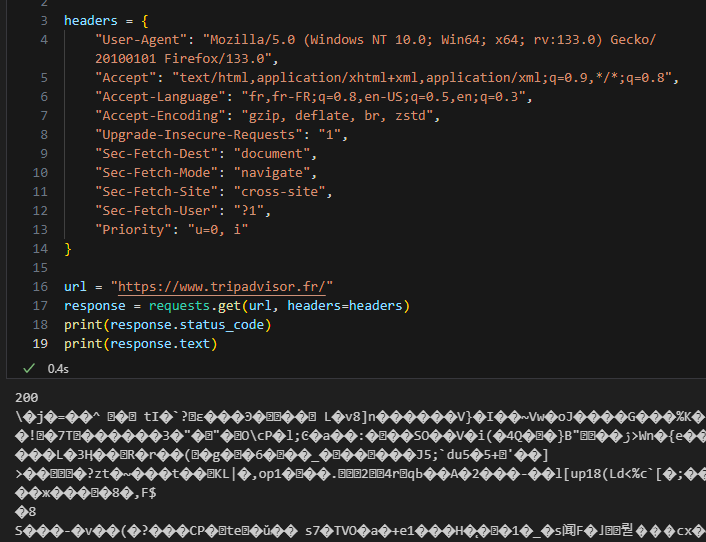
\includegraphics[scale=0.5]{Images/header2.png}
\captionof{figure}{La réponse du serveur n'est pas celle attendue.}
\label{header_reponse1}
\end{center}

La figure \ref{header_reponse1} montre que le header a bien fait son effet, que le serveur a accepté notre requête et nous a envoyé les informations attendues, ou presque. La réponse attendue aurait dû être du texte clair écrit en HTML mais on peut voir que ce n'est pas le cas. Les caractères imprimés n'ont aucun sens.

Dans notre header, on peut voir à la ligne \textit{Accept-Encoding} que plusieurs arguments ont été donnés. Ils indiquent au serveur sous quelle forme il peut nous envoyer les données demandées. Pour savoir laquelle a été retenue, il suffit de regarder dans le header de la réponse (Figure \ref{header_Brave}) pour y trouver la réponse. Le champs \textit{x-content-encoding-over-network} contient la valeur \textit{br}. La bibliothèque \textit{brotli} de Python permet alors de décoder le contenu de la réponse et on obtient bien le contenu HTML de la page visitée (Figure \ref{brotly}).

\begin{center}
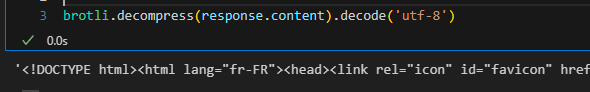
\includegraphics[scale=0.8]{Images/brotli.png}
\captionof{figure}{Enfin du texte lisible !}
\label{brotly}
\end{center}

Il est maintenant possible de récupérer les pages d'un site web comme tripadvisor.

\paragraph{Parsing :}

Le langage HTML est un langage structuré constitué de balises qui définissent le rôle de chaque élément dans la page. Il est possible de cibler les différents éléments qui constituent la structure la page. Il y a toutefois plusieurs problèmes :
\begin{itemize}
\item L'utilisation de la minification rend le fichier illisible
\item Le nombre de balises qui constituent la page rend la recherche "manuelle" dans le code source très difficile
\end{itemize}

\begin{center}
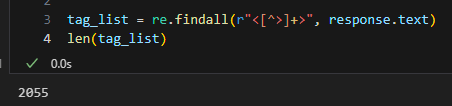
\includegraphics[scale=0.8]{Images/tag_list.png}
\captionof{figure}{2000 balises à parcourir pour identifier la structure d'une page...}
\label{tag_list}
\end{center}

La bibliothèque \textit{Beautiful Soup} offre une méthode pour palier au problème de la minification : prettify. Il est alors possible de parcourir le contenu du code source avec le confort d'une indentation claire.

Le problème de la quantité de balises en revanche ne peut qu'être contourné. Pour cela, on peut à nouveau utiliser les outils développeur de notre navigateur. Ils permettent de cibler un élément dans le rendu de la page et de trouver le bout de code qui y correspond.

\begin{center}
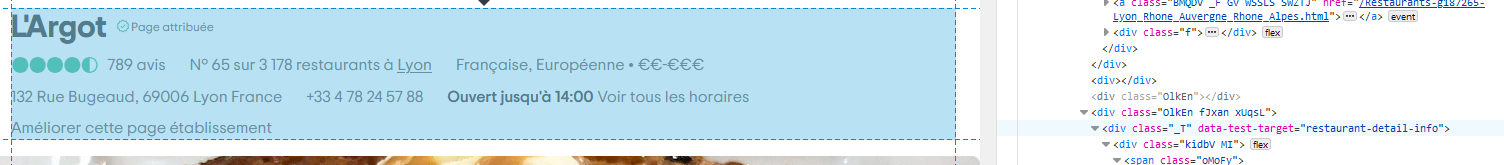
\includegraphics[scale=0.8]{Images/targeting_tag.png}
\captionof{figure}{Le Bandeau en début de page correspond ici à la balise div en surbrillance.}
\label{target_tag}
\end{center}

La figure \ref{target_tag} montre les attributs de la balise div qui contient l'ensemble du bandeau en surbrillance. Cliquer sur l'élément dans le rendu visuel permet de sélectionner la balise en question (figure \ref{div_content}).

\begin{center}
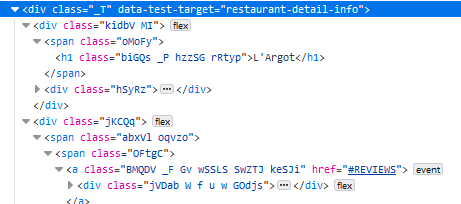
\includegraphics[scale=0.8]{Images/div_content.png}
\captionof{figure}{la balise div et une partie de son contenu.}
\label{div_content}
\end{center}

Il devient dès lors très facile de cibler un élément d'intérêt en particulier ,de le retrouver dans le code et d'identifier ses attributs. On vois dans la figure \ref{div_content} que cette balise div possède les attributs \textit{class} et \textit{data-test-target}.

C'est à partir du type de la balise, de ses attributs, de ses parents et enfants que l'on va pouvoir extraire l'ensemble des informations voulues à partir du code HTML d'une page web.

